% \chapter{Introduction}\label{chap:introduction}
\chapter{引言}\label{chap:introduction}
% Robotics celebrated its 50th birthday in 2011, dating back to the first commercial robot in 1961 (the Unimate). In a ``Tonight Show'' from the time, this robot did amazing things: it opens a bottle of beer, pours it, puts a golf ball into the hole, and even conducts an orchestra. This robot does all what we expect a good robot to do: it is dexterous, it is accurate, and even creative. Since this robot's appearance on the Tonight show, more than 50 years have passed --- so how incredible must be the capabilities of today's robots and what must they be able to do?

机器人在2011年庆祝了50岁生日,它的历史可追溯到1961年的第一个商业机器人Unimate。在当时的“今晚秀”中,这个机器人做了惊人的事情:它开啤酒,然后倒酒,把一个高尔夫球放进洞里,甚至指挥一个乐队。这个机器人完成了我们期望的一个优秀机器人能做的:它是灵巧的、它是准确的、甚至是创造性的。自这个机器人在“今晚秀”展出之后已经过去了五十多年,如今机器人的能力会如何的令人难以置信,以及它们能做什么呢?

% Interestingly, we just recently learned doing all the things demonstrated by Unimate autonomously. Unimate indeed did what was shown on TV, but all motions have been preprogrammed and the environment has been carefully staged.  Only the advent of cheap and powerful sensors and computation has recently enabled robots to detect an object by themselves, plan motions to it and grasp it. Yet, robotics is still far away from doing these tasks with human-like performance.

有趣的是,我们刚刚学会了如何自主地完成Unimate做的所有事情。Unimate确实做了电视上显示的,但是所有的动作都已经被预先编程,环境已经被仔细地分成多个阶段。廉价而强大的传感器和计算的出现使机器人能够自己检测到物体、规划动作接近并抓取它。然而,机器人技术离以类人的表现来完成这些任务仍很遥远。

% This book introduces you to the computational fundamentals of autonomous robots. Robots are \emph{autonomous} when they make decisions in response to their environment vs.\ simply following a pre-programmed set of motions. They achieve this using techniques from signal processing, control theory, and artificial intelligence, among others. These techniques are coupled with the mechanics, the sensors, and the actuators of the robot. Designing a robot therefore requires a deep understanding of both algorithms and its interfaces to the physical world.

本书向你介绍自主机器人的计算基础知识。当机器人根据自己的环境作出决定时,机器人是\emph{自主的(Autonomous)},而不是只执行预先设定的一组动作。他们使用信号处理、控制理论和人工智能等技术实现了这一点。这些技术与机器人力学、传感器和驱动器相结合。因此,设计机器人需要深入了解算法和机器人与物理世界的交互。

% The goals of this introductory chapter are to introduce the kind of problems roboticists deal with and how they solve it.

本章的目的是介绍机器人技术面临的问题以及它们如何解决这些问题。

% \section{Intelligence and embodiment}
\section{智能与实例}
% Our notion of ``intelligent behavior'' is strongly biased by our understanding of the brain and how computers work: intelligence is located in our heads. In fact, however, a lot of behavior that looks intelligent can be achieved by very simple means. For example, mechanical wind-up toys can avoid falling off an edge simply by using a fly-wheel that rotates at a right angle to their direction of motion and a caster wheel. Once the caster wheel loses contact with the ground---that is the robot has reached the edge---the fly-wheel kicks in and pulls the robot to the right (Figure \ref{fig:winduptoy}).

我们对“智能行为”的概念受到我们对大脑以及计算机的工作原理理解的很大影响:智能位于我们的大脑。然而,事实上很多看起来很智能的行为可以通过非常简单的方法来实现。例如,机械上弦玩具可以简单地通过使用与其运动方向成直角旋转的飞轮和脚轮来避免从边缘掉落。一旦脚轮与地面接触 -- 即机器人已经到达边缘 -- 飞轮立即启动并将机器人向右拉(图~\ref{fig:winduptoy})。

\begin{figure}
	\centering
		\includegraphics[width=\textwidth]{figs/winduptoysketch.png}
	% \caption{A wind-up toy that does not fall off the table using purely mechanical control. A fly-wheel that turns orthogonal to the robot's motion induces a right turn as soon as it hits the ground once the front caster wheel goes off the edge.}
	\caption{纯粹利用机械控制避免从桌上掉落的上弦玩具。一旦脚轮踏空,转动方向与机器人的运动方向正交的飞轮就会触地并立即使机器人向右转。}
	\label{fig:winduptoy}
\end{figure}

% A robot vacuum cleaner might solve the same problem very differently: it employs infrared sensors that are pointed downwards to detect edges such as stairs and then issues a command to make an avoiding turn. Once electronics are on-board, this is a much more efficient, albeit much more complex, approach.

机器人吸尘器可能会以截然不同的方式解决这个问题:它采用朝下的红外传感器来检测楼梯等边缘,然后发出转弯命令。将电子元件安装在主板上虽然复杂,但更有效率。

% Whereas the above examples provide different approaches to implement intelligent behaviors, similar trade-offs exist for robotic planning. For example, ants can find the shortest path between their nest and a food source by simply choosing the trail that already has more pheromones, the chemicals ants communicate with, on it. As shorter paths have ants not only moving faster towards the food, but also returning faster, their pheromone trails build up quicker (Figure \ref{fig:ants}). But ants are not stuck to this solution. Every now and then, ants give the longer path another shot, eventually finding new food sources. What looks like intelligent behavior at the swarm level, is essentially achieved by a pheromone sensor that occasionally fails. A modern industrial robot would solve the problem completely different: it would first acquire some representation of the environment in the form of a map populated with obstacles, and then plan a path using an algorithm.

上述例子提供了不同的实现智能行为的方法,机器人规划也存在类似的折中方案。例如,蚂蚁可以通过直接选择已经具有更多的信息素(蚂蚁用来通信的化学物质)的路径,找到它们的巢和食物源之间的最短路径。因为较短的路径使得蚂蚁向食物移动速度更快,返回速度更快,所以信息素路径更快建好(图~\ref{fig:ants})。 但是,蚂蚁并不一直执行这个方案。有时,蚂蚁会再次尝试更长的路并最终找到新的食物来源。这看起来像是群体智能行为,而事实上是由一个偶尔出错的信息素传感器导致的。一个现代工业机器人会截然不同地解决这个问题:它首先获取环境的一些表示(这种表示是填充有障碍物的地图形式),然后使用算法来规划路径。

\begin{figure}
	\centering
		
\includegraphics[width=\textwidth]{figs/ants.png}
	% \caption{Ants finding the shortest path from their nest (bottom) to a food source (top). From left to right: The ants initially have equal preference for the left and the right branch, both going back and forth. As ants return faster on the shorter branch there will be more pheromones present on the short branch once a new ant arrives from the nest(source?).}
	\caption{蚂蚁寻找从蚁巢(底部)到食物源(顶部)的最短路径。从左到右:蚂蚁最初对左右分支有同等的偏好,两者都是来回的。由于蚂蚁在较短的分支上返回速度更快,一旦新的蚂蚁从食物源返回蚁巢,短的分支上会有更多的信息素。}
	\label{fig:ants}
\end{figure}

% Which solution to achieve a certain desired behavior is best depends on the resources that are available to the designer. We will now study a more elaborate problem for which many, more or less efficient, solutions exist.

实现某种所需行为的最佳解决方案取决于设计者可用的资源。现在我们将研究一个更为复杂的问题,这个问题存在许多或高效、或低效的解决方案。

% \section{A roboticists' problem}
% Imagine the following scenario. You are a robot in a maze-like environment such as a cluttered warehouse, hospital or office building. There is a chest full of gold coins hidden somewhere inside. Unfortunately, you don't have a map of the maze. In case you find the chest, you may only take a couple of coins at a time, and bring them to the exit door where your car is parked.

\section{一个机器人研究者的问题}
想象下面的情况。你是一个机器人,处在一个像迷宫般的环境,比如仓库、医院或办公大楼。里面藏有一个装满金币的箱子。不幸的是,你没有迷宫的地图。如果你发现箱子,你一次只能拿几个金币,并把它们运到你停车的出口。

% \begin{framed}
% Think about a strategy that will allow you to harvest as many coins in the shortest time as possible. Think about the cognitive and perception capabilities you would make use of. Now discuss alternative strategies, if you would not have these capabilities, i.e., what if you were blind, had no memory?
% \end{framed}

\begin{framed}
想一个可以让你在尽可能短的时间内收获尽可能多的金币的策略。想想你将会使用的认知和感知能力。现在讨论替代策略,如果你不具备这些功能呢?即如果你看不到、没有记忆呢?
\end{framed}


% These are exactly the same problems a robot would have. A robot is a mobile machine that has sensors and computation, which allows it to reason about its environment. Current robots are far from the capabilities that humans have, therefore it makes a lot of sense to think about what strategies \emph{you} would employ to solve a problem, if you were lacking important perception or computational capabilities.

这是机器人会遇到的完全相同的问题。机器人是一种具有传感器和计算机的移动机器,这使它能对其环境进行推理。目前的机器人远没有人类的能力,因此如果缺乏重要的感知或计算能力,那么想想\emph{你}应该采取什么策略来解决问题,这是很有意义的。

% Before we move forward to discuss potential strategies for robots with impeded sensory systems, lets quickly consider an optimal strategy. You will need to explore the maze without entering any branch twice. You can use a technique known as \emph{depth-first search} to do this, but will need to be able to not only map the environment, but also localize in the environment, e.g., by recognizing places and dead-reckoning on the map. Once you have found the gold, you will need to plan the shortest path back to the exit, which you can then use to go back and forth until all the gold is harvested.

在我们进一步讨论有感知障碍系统的机器人的潜在策略之前,让我们快速考虑一个最佳策略。你探索迷宫但不能进入任何分支两次以上。你可以使用称为\emph{深度优先搜索(Depth-First Search,DFS)}的技术来执行此操作,但你不仅需要能对环境建图,还需要能够在环境中进行定位,例如通过识别地图上的位置进行推理。一旦找到金库,你需要规划回到出口的最短路径,然后你可以往返金库,直到获得所有的金币。

\section{Ratslife}\label{sec:ratslife}
% Ratslife is a miniature robot maze competition developed by Olivier Michel from Cyberbotics S.A. The Ratslife environment can easily be created from LEGO bricks, card board or wood and the game can be played with any two mobile robots, preferably ones with the ability to identify markers in the environment. These include simple differential-wheel educational platforms with onboard cameras or even a smart-phone driven robot. Figure \ref{fig:ratslife} shows a simple sample environment that can be constructed from craft materials and can be used to teach the practical aspects of mobile robots for competitions.

Ratslife是由Cyberbotics SA的Olivier Michel开发的微型机器人迷宫比赛。Ratslife环境可以轻松地使用乐高积木、纸板或木头创建,比赛可以由任何两个移动机器人一起进行,这些机器人最好具有识别环境中标记的能力。比如带有车载摄像头甚至智能手机驱动机器人的简易差速轮平台。图~\ref{fig:ratslife}显示了一个可以由工艺材料构建的简单样本环境,可以用它教授比赛移动机器人的实践部分。

\begin{figure}
	\centering
		\includegraphics[width=\textwidth]{figs/ratslife.png}
	% \caption{A simple maze made from cardboard, wood or Lego bricks with one or more charging stations. Locations in the maze are marked with unique markers that can be recognized by a simple robot.}
	\caption{装有一个或多个充电站的简单迷宫,由纸板、木头或乐高积木制成。迷宫中的位置标有独特的标记,可以被简易的机器人识别。}
	\label{fig:ratslife}
\end{figure}

% In RatsLife, two miniature robots  compete on searching for four ``feeders'' that are hidden in  a maze. Once a robot reaches a feeder, it receives ``energy'' to go on for another 60s, and the feeder becomes temporarily unavailable. After a short while, the feeder becomes available again. The feeders can be either controlled by a referee who also takes care of time-keeping or constructed as part of a simple curriculum on electronics or mechatronics.

在RatsLife中,两台微型机器人正在寻找隐藏在迷宫中的四个“充电站”。一旦机器人靠近“充电站”,它会获得“能量”继续运行60秒,然后这个“充电站”暂时不可用。短暂的一段时间后,“充电站”再次可用。“充电站”可以由负责计时的裁判负责,或者作为电子或机电课程的一部分来制作。

% It should be clear by now, how YOU would solve these tasks using your abilities, and you should have also thought about fall-back strategies in case some of your sensors are unavailable. Here are some possible algorithms for a robot, ordered after the capabilities that it provides:

现在应该清楚的是,你将如何使用你的能力来完成这些任务。如果你的某些传感器不可用,你还应该考虑回退策略。下面是一些可能的机器人算法,按照它们提供的功能进行排序:

% \begin{itemize}
% \item Imagine you have a robot that can only drive (actuation) and bounce off a wall. The resulting random walk will eventually let the robot reach a feeder. As the allowed time to do so is limited, it is likely that the robot's energy will soon deplete.
% \item Now imagine a robot that has a sensor that gives it the ability to estimates its distance from a wall. This could be a whisker, an infrared distance sensor, an ultra-sound distance sensor, or a laser range finder. The robot could now use this sensor to keep following a wall to its right. Using this strategy for solving the maze, it will eventually explore the entire maze except for islands inside of it.
% \item Finally, think about a robot that could identify simple patterns using vision, has distance sensors to avoid walls, and an ``odometer'' to keep track of its wheel rotations. Using these capabilities, a potential winning strategy would be to explore the environment, identify markers in the environment using vision and use them to create a map of all feeder locations, calculate the shortest path from feeder to feeder and keep going back and forth between them. Strategy-wise, it might make sense to wait just in front of the feeder and approach it only shortly before the robot runs out of power.
% \end{itemize}

\begin{itemize}
\item 想象一下,你有一个只能行驶(驱动)并遇墙折返的机器人。由此产生的随机游走将最终使机器人靠近一个“充电站”。由于允许的时间有限,机器人的能量可能会很快耗尽。
\item 现在想象一个带有有一个传感器的机器人,它能够估计离墙的距离。这可以是触须传感器、红外距离传感器、超声距离传感器或激光测距仪。现在机器人可以使用这个传感器来沿着右侧的墙壁行驶。使用这个策略来探索迷宫,它将最终遍历除了迷宫中孤立部分的整个迷宫。
\item 最后,考虑一个可以使用视觉识别简单图案的机器人,它装有避开墙壁的距离传感器和跟踪其轮转的“里程计”。使用这些功能的潜在获胜策略是探索环境,使用视觉识别环境中的标记,并使用它们来创建有所有“充电站”位置的地图,计算从“充电站”到“充电站”的最短路径,并在它们之间来回移动。除此之外,机器人在能量耗尽之前不久,直接到“充电站”身边等待可能更合理。
\end{itemize}

% \section{Challenges of Mobile Autonomous Robots}
\section{移动自主机器人的挑战}

% Being able to stitch sensor information together to map the environment just by counting your own steps and orienting yourself by using distinct features of the environment is known as Simultaneous Localization and Mapping (SLAM). The key challenge here is that the length of the steps you take are uncertain (a wheeled robot might slip or have slightly differently sized wheels, e.g.) and it is not possible to recognize places with 100\% accuracy (not even for a human). In order to be able to implement something like the last algorithm on a real robot, we will therefore need to understand

整合传感器信息,通过计数行进步数创建环境的地图并通过使用不同的环境特征来定位,称为同步定位与建图(SLAM)。这里的关键挑战在于,你所得到的距离是不确定的(例如,轮式机器人可能滑动或略有不同大小的车轮),并且无法100$\%$识别位置(甚至人也做不到)。为了能够在真正的机器人上实现上述算法,我们需要理解:

% \begin{itemize}
% \item How does a robot move? How does rotation of its wheels affects its position and speed in the world?
% \item How do we have to control the wheel-speed in order to reach a desired position?
% \item What sensors exist for a robot to perceive its own status and its environment?
% \item How can we extract structured information from a vast amount of sensor data?
% \item How can we localize in the world?
% \item How can error be represented and how can we reason in the face of uncertainty?
% \end{itemize}

\begin{itemize}
\item 机器人如何移动?轮子的旋转如何影响机器人在环境中的位置和速度?
\item 我们如何控制车轮速度以到达所需的位置?
\item 机器人有哪些传感器可以感知到自己的状态和环境?
\item 我们如何从大量的传感器数据中提取结构化信息?
\item 我们如何在环境中定位?
\item 如何表示误差,面对不确定性如何推理?
\end{itemize}

% In order to answer these questions, we will rely on trigonometry, linear algebra, and probability theory. Specific concepts that will be used throughout this book are basic trigonometry, matrix notation, Bayes' formula, and the concept of probability distributions. You will see that robotics is actually a great vehicle to add meaning to these concepts!

我们将依靠三角学、线性代数和概率理论来回答这些问题。本书使用的具体概念是基本三角学、矩阵表示法、贝叶斯公式和概率分布。你会看到机器人实际上是一个很好的工具来增加这些概念的意义!


% \section{Challenges of Autonomous Manipulation}
\section{自主操作的挑战}

% Think about the last time you worked with your hands. This includes typing on your keyboard, writing on a piece of paper, sewing a button onto a shirt, and using a hammer or a screwdriver. You will notice that these activities require a wide range of dexterity, that is the ability to manipulate objects with precision, a wide range of forces, and a wide range of sensorial capabilities. You will also notice that some tasks go beyond your capabilities, such as putting yarn through a hole in fabric, grasping a screw, or driving a nail into a piece of wood, but can be easily solved with the right tool.

想想你最后一次用你的手。这包括在键盘上打字、在纸上书写、将纽扣缝在衬衫上、以及使用锤子或螺丝刀。你会注意到这些活动需要很大的灵活性,也就是精确地操纵物体、不同的力度和各种各样的感知的能力。你还会注意到某些任务超出了你的能力,例如将纱线穿过织物孔、抓住螺丝、或将钉子钻入木头,但是这些可以使用正确的工具轻松解决。

% So far, robotic hands are far from reaching the dexterity of a human hand. Yet, with the right tool (called ``end-effector'' in robotics speech) \index{End-effector} some tasks can be solved even better, that is faster and more precisely, than by humans. As for solving a mobile robotics problem, manipulation problems require you to think about the right mix of reasoning and mechanism design. For example, grasping tiny parts might be impossible with tweezers, but really easy when using a sucking mechanism. Or, picking up a test tube that is hardly visible with the robots' sensors can be picked up almost blindly when using a funnel-like mechanism at your end-effector. Unfortunately, these tricks will most likely limit the versatility of your robot, requiring you to think about the problem and the users's need as a whole.

到目前为止,机器人手远远没有达到人手的灵巧度。然而,使用正确的工具(在机器人术语中称为“末端执行器(End-effector)”)\index{末端执行器(End-effector)}某些任务可以比人类更快更精确地完成。对于解决移动机器人问题,操作问题需要考虑正确地结合推理和机制设计。例如,有时使用镊子抓取微小的部件是不可能的,但如果使用吸吮机制就会很容易。或者,要拾起机器人传感器几乎“看不见”的试管,当末端执行器使用类似漏斗的机制时,可以毫不费力地拾起。不幸的是,这些技巧很可能会限制机器人的多功能性,需要统筹考虑问题和用户的需求。


%% Start - Was commneted, Sep 5, 2017
% \section{The first industrial robot ``Unimate"}
% Since the introduction of the first industrial robot ``Unimate'' in 1961, the robotics industry classically consists of static manipulators that perform repetitive tasks such as welding or part placement, as well as of remote controlled machines for exploring hazardous areas. Recent advances in sensor technology and artificial intelligence are quickly enabling a new kind of robotic system: robots that can make autonomous decisions. The most prominent example of this class of robots is iRobot's ``Roomba'' vacuum cleaner that was introduced in 2002 and that uses a variation of algorithm \#1 above to solve the floor cleaning problem due to the lack of sophisticated sensors and computation. More recently, SLAM has found its ways into cars, university teams winning the DARPA Grand Challenge, Google's cars logging more than 140,000 miles, and Volkswagen presenting the first assisted driving system in 2011. Similarly, KIVA systems  successfully distributes mobile robots for automatic warehouses. These robots are still remote controlled and operate in constrained environments that provide them the ability to localize and reason on a simplified representation of the world - all items in the KIVA world are living on a grid. Novel sensors such as the xBox Kinect that provide 3D depth measurements at unprecedented low cost, increasingly capable and cheap computers, and a better understanding on how to reason about uncertainty will enable a large number of applications raising from autonomous warehouse helpers, home and elderly care, robotic toys and many other gimmicks straight from the Jetsons very soon.
%% End - Was commneted, Sep 5, 2017


% \section*{Take-home lessons}
\section*{课后补充}
% \begin{itemize}
% \item How to best solve a problem is a function of the available sensing, actuation, computation and communication abilities of the available platform. Usually, there exist trade-offs that allow you to solve a problem using a minimal set of resources, but compromise performance such as speed, accuracy or reliability.
% \item Robotics problems are different from problems in pure Artificial Intelligence, that do not deal with unreliable sensing or actuation.
% \item The unreliability of sensors, actuators and communication links require a probabilistic notion of the system and reason with uncertainty.
% \end{itemize}

\begin{itemize}
\item 如何最好地解决问题是机器人平台可用的感知、驱动、计算和通信能力的综合。通常存在折中,允许你使用最少的资源来解决问题,但会影响性能,如速度、准确性或可靠性。
\item 机器人问题不同于纯人工智能中的问题,它需要处理不可靠的感知或驱动。
\item 传感器、驱动器和通信链路的不可靠性需要系统的概率定义,然后对不确定性进行推导。
\end{itemize}


% \section*{Exercises}\small
% \begin{enumerate}
% \item What kind of sensors do you need to solve the ``Ratslife'' game? Think both about trivial and close-to-optimal approaches.
% \item What devices in your home could be considered robots? Why and why not?
% \item Which industries have been recently revolutionized by robotics? Into which industries were robots introduced first?
% \item What sensors are you using when grasping an object? Enumerate them all. Which ones are absolutely necessary for good performance?
% \item Think about robots vacuuming your floor or mowing your lawn. Do they use any planning? Why or why not?
% \item What kind of sensors would you need in a car that drives completely autonomously? Think first about the kind of information that the car needs to be aware of and then discuss possible sensors that could capture this information.
% \item Implement a simple line-following using a robot of your choice. How does the thickness of the line affect the sensor placement on the robot? How does its curvature affect the robot's speed?
% \item Implement a maze solving algorithm that uses simple wall-following using a robot of your choice. How does the sensor geometry affect the robot's performance? What are the parameters that you find yourself tuning?
% \end{enumerate}\normalsize

\section*{习题}\small
\begin{enumerate}
\item 你需要什么样的传感器才能完成“Ratslife”游戏?考虑一般的和接近最优的方法。
\item 你家中的哪些设备可以被认为是机器人?为什么是或者不是?
\item 哪些行业最近被机器人革命化了?机器人会先被引入到哪些行业?
\item 抓取物体时使用什么传感器?为了达到好的性能,列举哪些是绝对必要的?
\item 想想机器人为你打扫地板或割草坪。他们是否有任何规划?为什么是或者不是?
\item 你需要什么样的传感器来实现完全自主驾驶汽车?首先考虑汽车需要获取的信息,然后讨论获取这些信息的可能的传感器。
\item 用你选择的机器人实现简单的线条跟踪。线条的宽度如何影响机器人上传感器的位置?它的曲率如何影响机器人的速度?
\item 用你选择的机器人实现简单的墙壁跟踪来解决迷宫问题。传感器几何如何影响机器人的性能?你发现你调整了哪些参数?
\end{enumerate}\normalsize


%% Start - Was commneted, Sep 5, 2017
%Robotics celebrated its 50th birthday in 2011, dating back to the first commercial robot in 1961 (the Unimate). In a ``Tonight show'' from the time, this robot did amazing things: its opening a bottle of beer, pouring it, putting a golf ball into the hole, and even conducting an orchestra. This robot does all what we expect a good robot to do: its dexterous, its accurate, and even creative. Since this robots appearance on the Tonight show more than 50 years have passed --- so how incredible must be the capabilities of today's robots and what must they be able to do?
%
%Interestingly, we just recently learned doing all the things demonstrated by Unimate autonomously. Unimate indeed did what was shown on TV, but all motions have been pre-programmed and the environment has been carefully staged.  Only the advent of cheap and powerful sensors and computation has recently enabled robots to detect an object by themselves, plan motions to it and grasp it. Yet, robotics is still far away from doing these tasks with human-like performance. Environments still need to be heavily staged for a robot to operate, and some objects are easier to work with than others. For example, ``Rollin' Justin'' is demonstrating skills very similar to those shown by the Unimate, but is able to perceive and reason about its environment:
%
%This works as follows: the robot perceives its environment with a sensor that generates 3D range data, such as stereo-vision, a sweeping laser scanner or an xbox Kinect. The robot creates a 3D representation of its environment that is relative to its own coordinate system. The robot now plans its motion using this 3D representation. This can be seen in the inset to the top right when the robot is manipulating items on the table. Detecting objects in the environment, matching them to their 3D model, and finding feasible grasp points are still major research challenges.
%
%The ``sense-plan-act'' paradigm, that is obtaining a 3D model of the world, planning therein, and consequently executing actions is not the final solution, however. Do humans really do this when performing complex manipulations? Rather not. Instead, we are relying on vision feedback or the sense of touch when performing a grasp. (Try to grasp an object after putting your hand on an ice block, temporarily impeding your sense of touch.)
%
%This class builds up on ``Introduction to Robotics'' and introduces current solutions to these problems. We will learn advanced concepts in robotic kinematics, such as car-like steering and inverse kinematics of high-DOF manipulators, feature recognition, RGB-D perception, visual servoing and SLAM. We will also learn to use state-of-the-art tools that allow you to model, visualize and control your robot. You will work with a 7-DOF manipulator arm both in simulation and using real hardware. The development environment consists of Ubuntu Linux, ROS and OpenCV that are available as VirtualBox. The real manipulator arm is available for experimentation in the lab. We will perform laboratory experiments - that can be mostly prepared and executed in simulation - that will introduce the tools and methods we are using and guide you toward an independent project.
%
%The class consists of homework assignments (experiments) and a team project. The final deliverable for the team project is a 3 page (5 pages) for undergraduates (graduate students). Your team project needs to articulate a hypothesis (what do you want to show?) that is validated experimentally on physical hardware. In order to prepare you for this, each laboratory exercise will require analysis of experimental data rather than submission of code.
%% End - Was commneted, Sep 5, 2017